\documentclass{article}

\usepackage{graphicx}
\graphicspath{ {./images/} }

\usepackage{authblk}
\usepackage{amsmath}

\begin{document}

\title{Autonomous Driving Car Simulator}
\author[1]{Bram Hagens}
\author[1]{Hidde Agterberg}
\affil[1]{Isendoorn College, Warnsveld}
\date{November 19, 2018}
\maketitle
\newpage

\tableofcontents
\newpage

\section{Abstract}
This project involves the creation of a simulation of an autonomous car that can learns in ways similar to how humans learn. The car has sensors that can detect distances to the objects in front and to the side of it and is controlled by an artificial neural network that gives steering inputs based on what the sensors see. The final product is capable of driving around in an enclosed environment without human interaction.
\newpage

\section{Introduction}
More than ninety percent for motor vehicle crashes are caused by human error[2]. Many companies are pushing towards fully autonomous cars with the hope that they will save lives by getting involved in fewer incidents resulting in fewer injuries. One of most well known commercial companies which creates fully autonomous cars is Tesla[7]. Fully autonomous vehicles, also known as Automation Level 5 vehicles[5], are capable of driverless operation under all circumstances. Because the vehicles need to be road ready, they need to be able to drive in a very wide range of environments. This paper is an attempt on creating such Level 5 autonomous vehicle in a simulated environment.

\section{Aim}
The aim of this project is to create a simulated self-learning autonomous vehicle, that successfully drives around a track surrounded by walls using only sensors to navigate around.

\section{Hypothesis}
With knowledge on specific machine learning techniques, the chance of creating a fully autonomous vehicle is significant. 

\newpage

\section{Theory}
\subsection{Simulator}
To build the simulator, Unity was used. Unity is a game engine, it enables people to make more complicated games or interactive simulators a lot quicker and less complicated. The engine uses a graphical interface with predefined objects, graphics and physics. In order to make the environment act/react, the user needs to program this manually using the Unity API (application programming interface, functions that make it easier to interact with the main program). Unity also has an asset store where people can download free or paid assets like vehicles, environments, characters and other props. 

\begin{center}
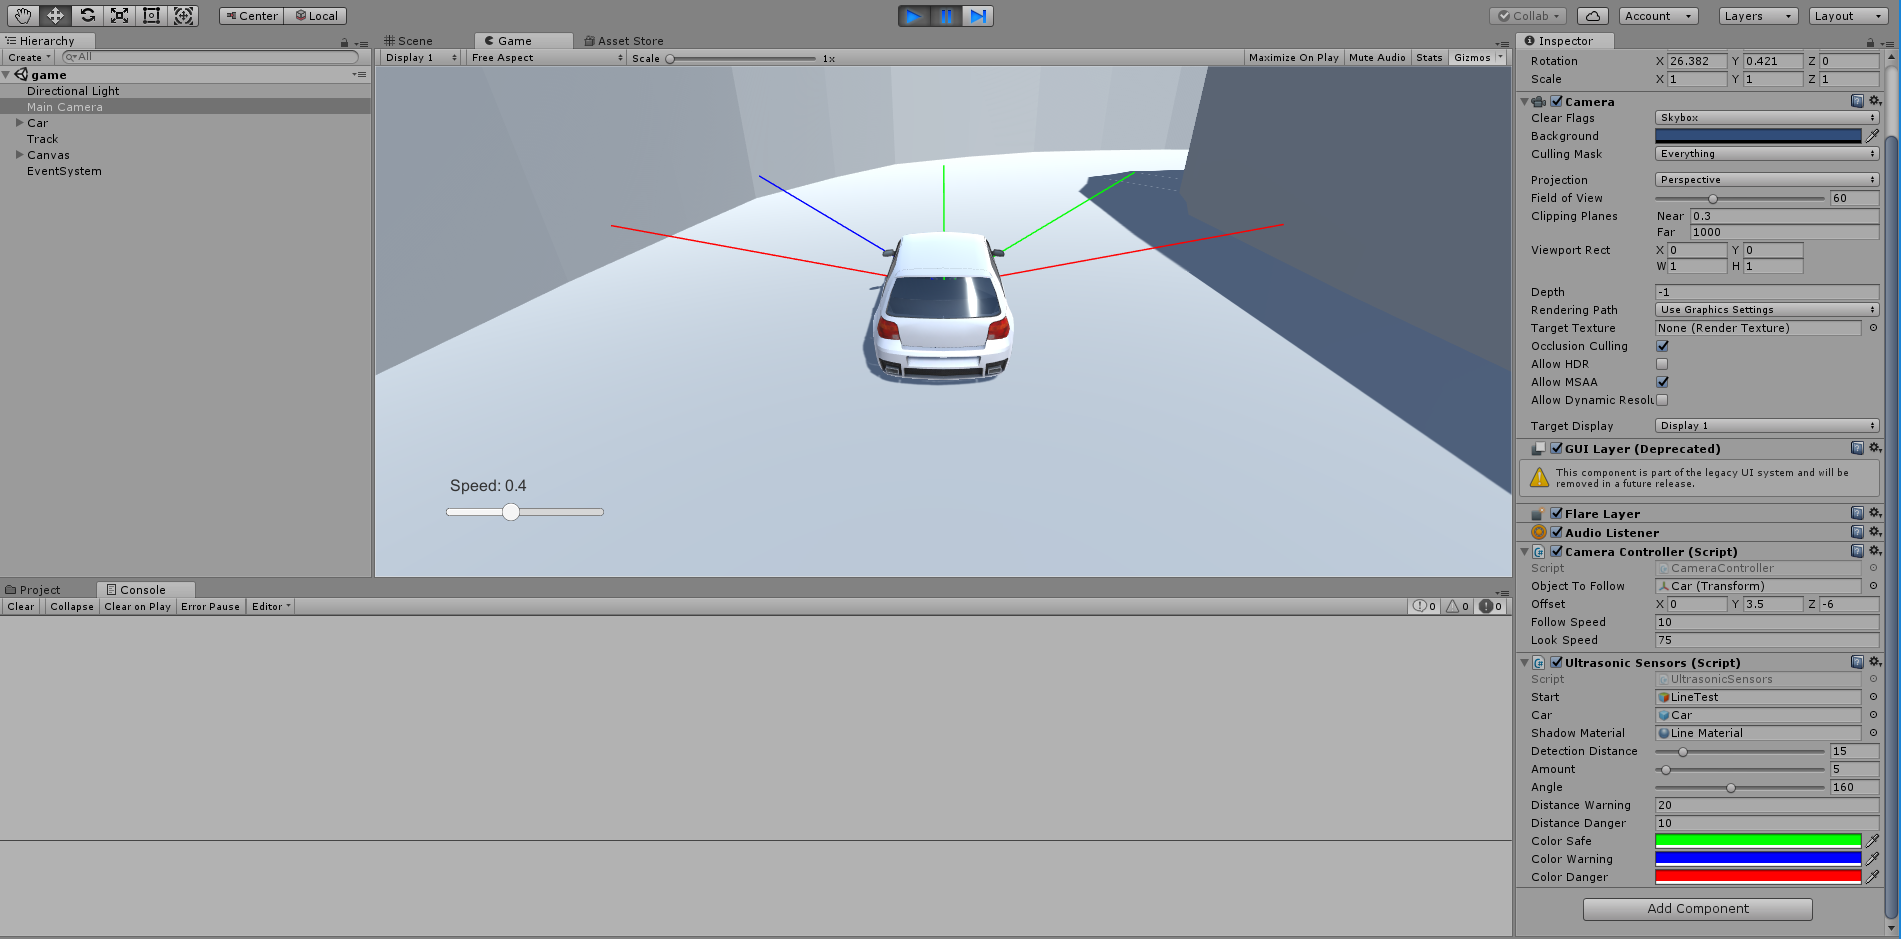
\includegraphics[width=\linewidth]{simulator_env}
\end{center}

\subsection{Inter-process communication}
To communicate between the simulator and the reinforcement learning network, User Datagram Protocol (UDP) is used. Packets of data are sent between the simulator and the network without much overhead, this is because UDP does not wait for delayed packets nor checks if the packets contain malformed or corrupt information. Other protocols such as TCP are more reliable as UDP, because there will be multiple attempts to deliver all packets, if some information is lost along the way it will be sent again. This is not ideal for this project, because it adds a lot of extra overhead, meaning there will be a longer delay between sending and receiving a packet, and a single missing packet is not having any significant effect on the result.

\subsection{Machine learning}
Machine learning is letting a computer behave in a way that would be described as learning if done by humans or animals[4]. This means a computer can learn something from data without being explicitly programmed to do. An artificial neural network is a common way to implement machine learning, these networks of neurons (also referred to as nodes) are a simulation of  the human brain. 

\begin{center}
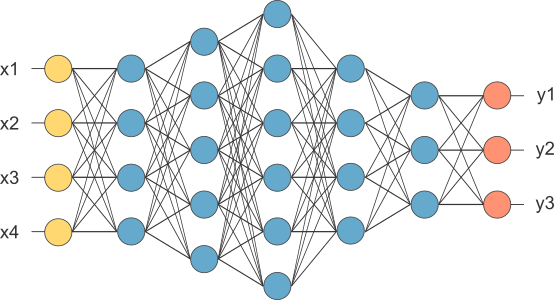
\includegraphics[width=\linewidth]{neural_net}
\end{center}

\begin{flushleft}
Figure 1[1]. The above example picture shows a visual representation of a neural network, a graph of linked nodes. The network starts with some input and uses matrix multiplications to calculate an output. 
\end{flushleft}

\subsection{Reinforcement learning}
Reinforcement learning is an area of machine learning where an agent takes actions to maximize a reward inside of an environment. 

\begin{flushleft}
The agent is defined as an object which can take actions, examples of these actions are steering left or accelerating. 
\end{flushleft}

\begin{flushleft}
The environment in the world in which the agent takes its actions, in this case the environment is a road. The environment is defined as the following function:  where  is the current state,  is the action the agent took. The function returns a tuple of the reward () and the next state ().
\end{flushleft}

\begin{flushleft}
The state is a concrete and immediate situation in which the agent finds itself, this includes a specific place and moment.
\end{flushleft}

\begin{flushleft}
The reward is the feedback, either positive or negative, given to the agent with which the success or failure of the agent’s actions can be measured.
\end{flushleft}

\begin{center}
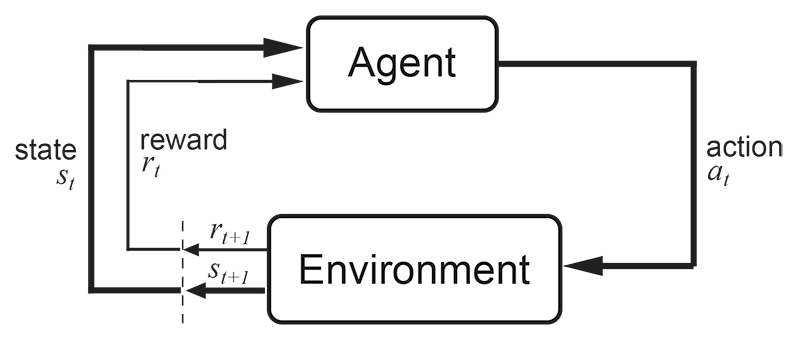
\includegraphics[width=\linewidth]{reinforcement_learning}
\end{center}

\begin{flushleft}
Figure 2[3]. The agent-environment loop. The environment gives the agent a state (st), the agent takes an action (at) based on the state, the environment rewards (rt+1) the agent appropriately according to the action and also sends the next state (st+1) and the loop repeats itself.
\end{flushleft}

\begin{flushleft}
The agent takes actions based on a policy, , using the state. This policy can be described as the probability of taking an action  for the given state . 
\end{flushleft}

\subsection{Q-learning}
Q-learning is a technique used in reinforcement learning. The goal of the technique is to learn a policy which tells the agent which actions it should take for the given state. 

\begin{flushleft}
With Q-learning, a Q-table, a simple lookup table, is created. In this table, the maximum expected rewards for each action at each state is stored. The table is initialized with zeros and later updated with calculated Q-values.
\end{flushleft}

\begin{flushleft}
The Q-learning algorithm is the following:
\begin{enumerate}
\item Initialize Q-table
\item Repeat:
\begin{enumerate}
\item Choose an action
\item Perform action
\item Measure reward of action
\item Update Q-table
\end{enumerate}
\end{enumerate}
\end{flushleft}

\begin{flushleft}
Step 1. Initialize Q-table
To store the Q-values, a Q-table has to be build. The amount of columns is equal to the amount of actions, the amount of rows is equal to the number of states. All values will be initialized with 0.
\end{flushleft}

\begin{flushleft}
Step 2. Repeat
All actions below are repeated until the training is stopped.
\end{flushleft}

\begin{flushleft}
Step 2a. Choose an action
Choose the best action in the current state. If every Q-value is equal to zero, an action is chosen at random using the epsilon greedy strategy. This strategy uses a number, epsilon, that is equal to 1 in the beginning. When an action needs to be chosen, a random number between 0 and 1 is generated. If this number is larger than epsilon, exploitation (choosing the best action) will be used. If the number is smaller than epsilon, exploration (choosing a random action) will be used. As the agent trains, epsilon will reduce progressively towards 0.
\end{flushleft}

\begin{flushleft}
Step 2b. Perform action
The action chosen in step 2a will be performed.
\end{flushleft}

\begin{flushleft}
Step 2c. Measure reward of action
After the action is performed, the reward and the new state are stored. 
\end{flushleft}

\begin{flushleft}
Step 2d. Update Q-table 
The Q-value is updated according to the Bellman equation:
\newline
\end{flushleft}

\begin{flushleft}
After a lot of iterations, the Q-table is able to solve the problem it was trained for.
\end{flushleft}

\begin{center}
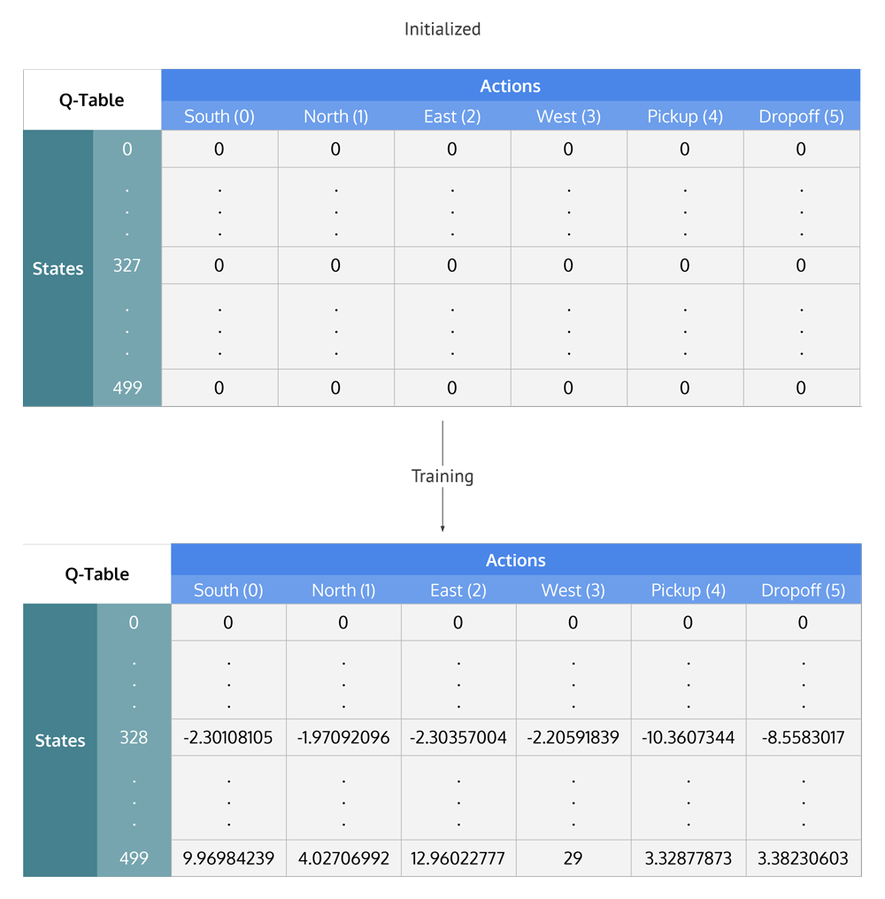
\includegraphics[width=\linewidth]{q_table}
\end{center}

Figure 5[8] Q-Tables during the initialization and training. The columns are the actions and the rows are the states. 

\subsection{Deep Q-learning}
Deep Q learning is a specific variation of Q learning. Where normal Q learning uses a Q table, deep Q learning makes use of a neural network (from deep learning). Like a lot of deep learning algorithms, deep Q learning improves its knowledge by calculating a loss and using backpropagation to update the weights. 

The deep Q learning algorithm is the following:
\begin{enumerate}
\item Initialize the memory
\item Initialize the weights 
\item For every episode:
\begin{enumerate}
\item Choose an action from the current state
\item Take the action, get the reward and next state
\item Store the experience
\item Take a sample of experience
\item Set the target Q
\item Update the weights
\end{enumerate}
\end{enumerate}

\begin{flushleft}
Step 1: Initialize the memory
The deep Q learning algorithm uses stored experience from the past, however when staring of it has no experience yet. This is why the experience memory first needs to be filled before the agent can start learning. It does this by taking an x amount of random actions and storing the information it got from those actions. Therefore the memory is made up out of a maximum amount of objects, these objects have the following structure: 
[state, action took, reward, next state].
\end{flushleft}

\begin{flushleft}
Step 2: Initialize the weights
The idea behind deep learning is that the neural network is initialized with random weights and biases, with training these weights and biases are slightly changed to minimize the loss and improve the accuracy. 
\end{flushleft}

\begin{flushleft}
Step 3: Episodes
The agent is told to train for a x amount of episodes, an episode lasts until the car crashes. In theory the more episodes: the better the agent gets at its task.
\end{flushleft}

\begin{flushleft}
Step 3a: Choosing an action 
To make sure the agent explores the environment, the algorithm uses the epsilon greedy strategy[9]. This strategy means that the agent will take random a random action if the explore probability is greater than an random number between zero and one. The explore probability can be calculated in the following way: 

explorep =explorestop+(explorestart-explorestop)exp(-decayratestep)
\newline

Where:
\begin{itemize}
\item explorep is the exploration probability 
\item explorestop is the minimum probability of taking a random action
\item explorestart is the starting probability of taking a random action
\item decayrate is the rate at which the exploration probability decreases
\item step is the step taken in all of the episodes
\item If the explore probability is smaller than the random number, the neural network will calculate an action.
\end{itemize}
\end{flushleft}

\begin{flushleft}
Step 3b: Take the action
The action from step 3a is now going to be taken. After the agent has taken the action it will retrieve a reward and the next state. 
\end{flushleft}

\begin{flushleft}
Step 3c: Store the experience
The experience ([state, action, reward, next state]), obtained by taking the action, is stored in the experience memory. If the memory is full, it will erase a part of the beginning of the array, to ensure space for the new experience.
\end{flushleft}

\begin{flushleft}
Step 3d: Take a sample of experience
The data to train the agent will be taken from the already obtained experience. The agent will take a random x sized batch of the objects from the experience memory. 
\end{flushleft}

\begin{flushleft}
Step 3e: Set the target Q
With the random batch of experience, the model can calculate the target Q values. The target Q, also called the max Q, is the maximum possible Q value for the next state[11]. To calculate a target Q value the following function is used:

targetq=reward+(max(Q))

Where:
reward is the reward from the random batch of experience
is the discount rate (the larger the discount is, the more the agent is going to focus on the long term reward[10])
Q is the output (or Q value) from the neural network with a certain input
\end{flushleft} 

\begin{flushleft}
Step 3f: Update the weights
In order to improve when training the agent needs to update its weights. The formula for updating a single weight is[11]:

newweight=(targetq -qvalue)wqvalue
\newline

Where:
\begin{itemize}
\item is the learning rate 
\item targetq is the calculated value in step 3e
\item qvalue is the output (or Q value) from the neural network with a certain input
\item w is the derivative of the current weight
\end{itemize}
\end{flushleft}

\subsection{Policy gradients}
Policy gradients are policy algorithms used in reinforcement learning. To get the highest rewards, the policy has to be optimal. The policy method is defined as  with theta as parameter, this means to find the optimal policy, the value of theta has to be optimal. A score function can determine how good theta is. This is done by taking the sum of all discounted rewards, a discounted reward is the normal reward multiplied by the factor gamma to account for the influence of the individual reward. The mathematical representation of the score function is [6]. 

\begin{flushleft}
Maximizing the value function can be done by using gradient descent. This becomes an easy task using the Policy Gradient Theorem[6].  can be written as , where  are all states and actions. Taking the gradient of this gives the following formula: . The optimal value is the maximum, this can be found by taking the derivative of the function: . This means that theta can be updated for each episode using the following formula , with alpha as the learning rate that influences how important this update in theta is. This means that to optimize a policy, a lot of training is needed.
\end{flushleft}

\section{Implementation}
\subsection{Requirements}
\subsection{Method}
\subsection{Pictures}

\section{Results}
\subsection{Q-learning}
\subsection{Deep Q-learning}
\subsection{Policy gradients}

\section{Proccessing Results}
\subsection{Q-learning}
\subsection{Deep Q-learning}
\subsection{Policy gradients}

\section{Discussion}

\section{Conclusion}

\section{Sources}

\begin{thebibliography}{9}
\bibitem{latexcompanion} 
Michel Goossens, Frank Mittelbach, and Alexander Samarin. 
\textit{The \LaTeX\ Companion}. 
Addison-Wesley, Reading, Massachusetts, 1993.
 
\bibitem{einstein} 
Albert Einstein. 
\textit{Zur Elektrodynamik bewegter K{\"o}rper}. (German) 
[\textit{On the electrodynamics of moving bodies}]. 
Annalen der Physik, 322(10):891–921, 1905.
 
\bibitem{knuthwebsite} 
Knuth: Computers and Typesetting,
\\\texttt{http://www-cs-faculty.stanford.edu/\~{}uno/abcde.html}
\end{thebibliography}

\section{Appendix}
\subsection{Simulator vs real car}
\subsection{Communicating between the simulator and the neural network}
\subsection{What kind of information to give to the neural network}
\subsection{Measuring the distance between the car and objects}
\subsection{Q learning vs deep Q learning vs policy gradients}

\end{document}